\subsection{Comparing the simulated system to the original data}

To create reusable algorithms for the simulated data, the concept of a slice is introduced. A slice is a two dimensional datastructure holding the value of the enhancement using $x$ and $y$ coordinates. These coordinates correspond to the $x$ and $y$ coordinates of the overal simulation but don't have to correspond to a plane with respect to the $z$ direction. Instead slices can be any geometric structures representable as $z=f(x,y)$. The local enhancement at these slices is only accounting for the electric field component $\mathbf{E}$ that is parallel to the slice surface. For slices along the $z$ axis this means discarding the $z$ component of the field, for more complex surfaces the field has to be projected on the surface for every value.

Figure \ref{fig:slices} shows plots of slices of the enhancement in the $xy$ plane using equidistant steps along the $z$ axis to illustrate the enhancement for different values of $z$. Noticeable are the fragments of spatial discretisation along the rounded gold structures.Light polarization along the dimer axis is assumed. The near field in the cavity between the gold nano disks contributes the biggest amount to the total enhancement. Above the structure ($z>\SI{45}{nm}$) the enhancement drops off significantly.

\begin{figure}[!h]
  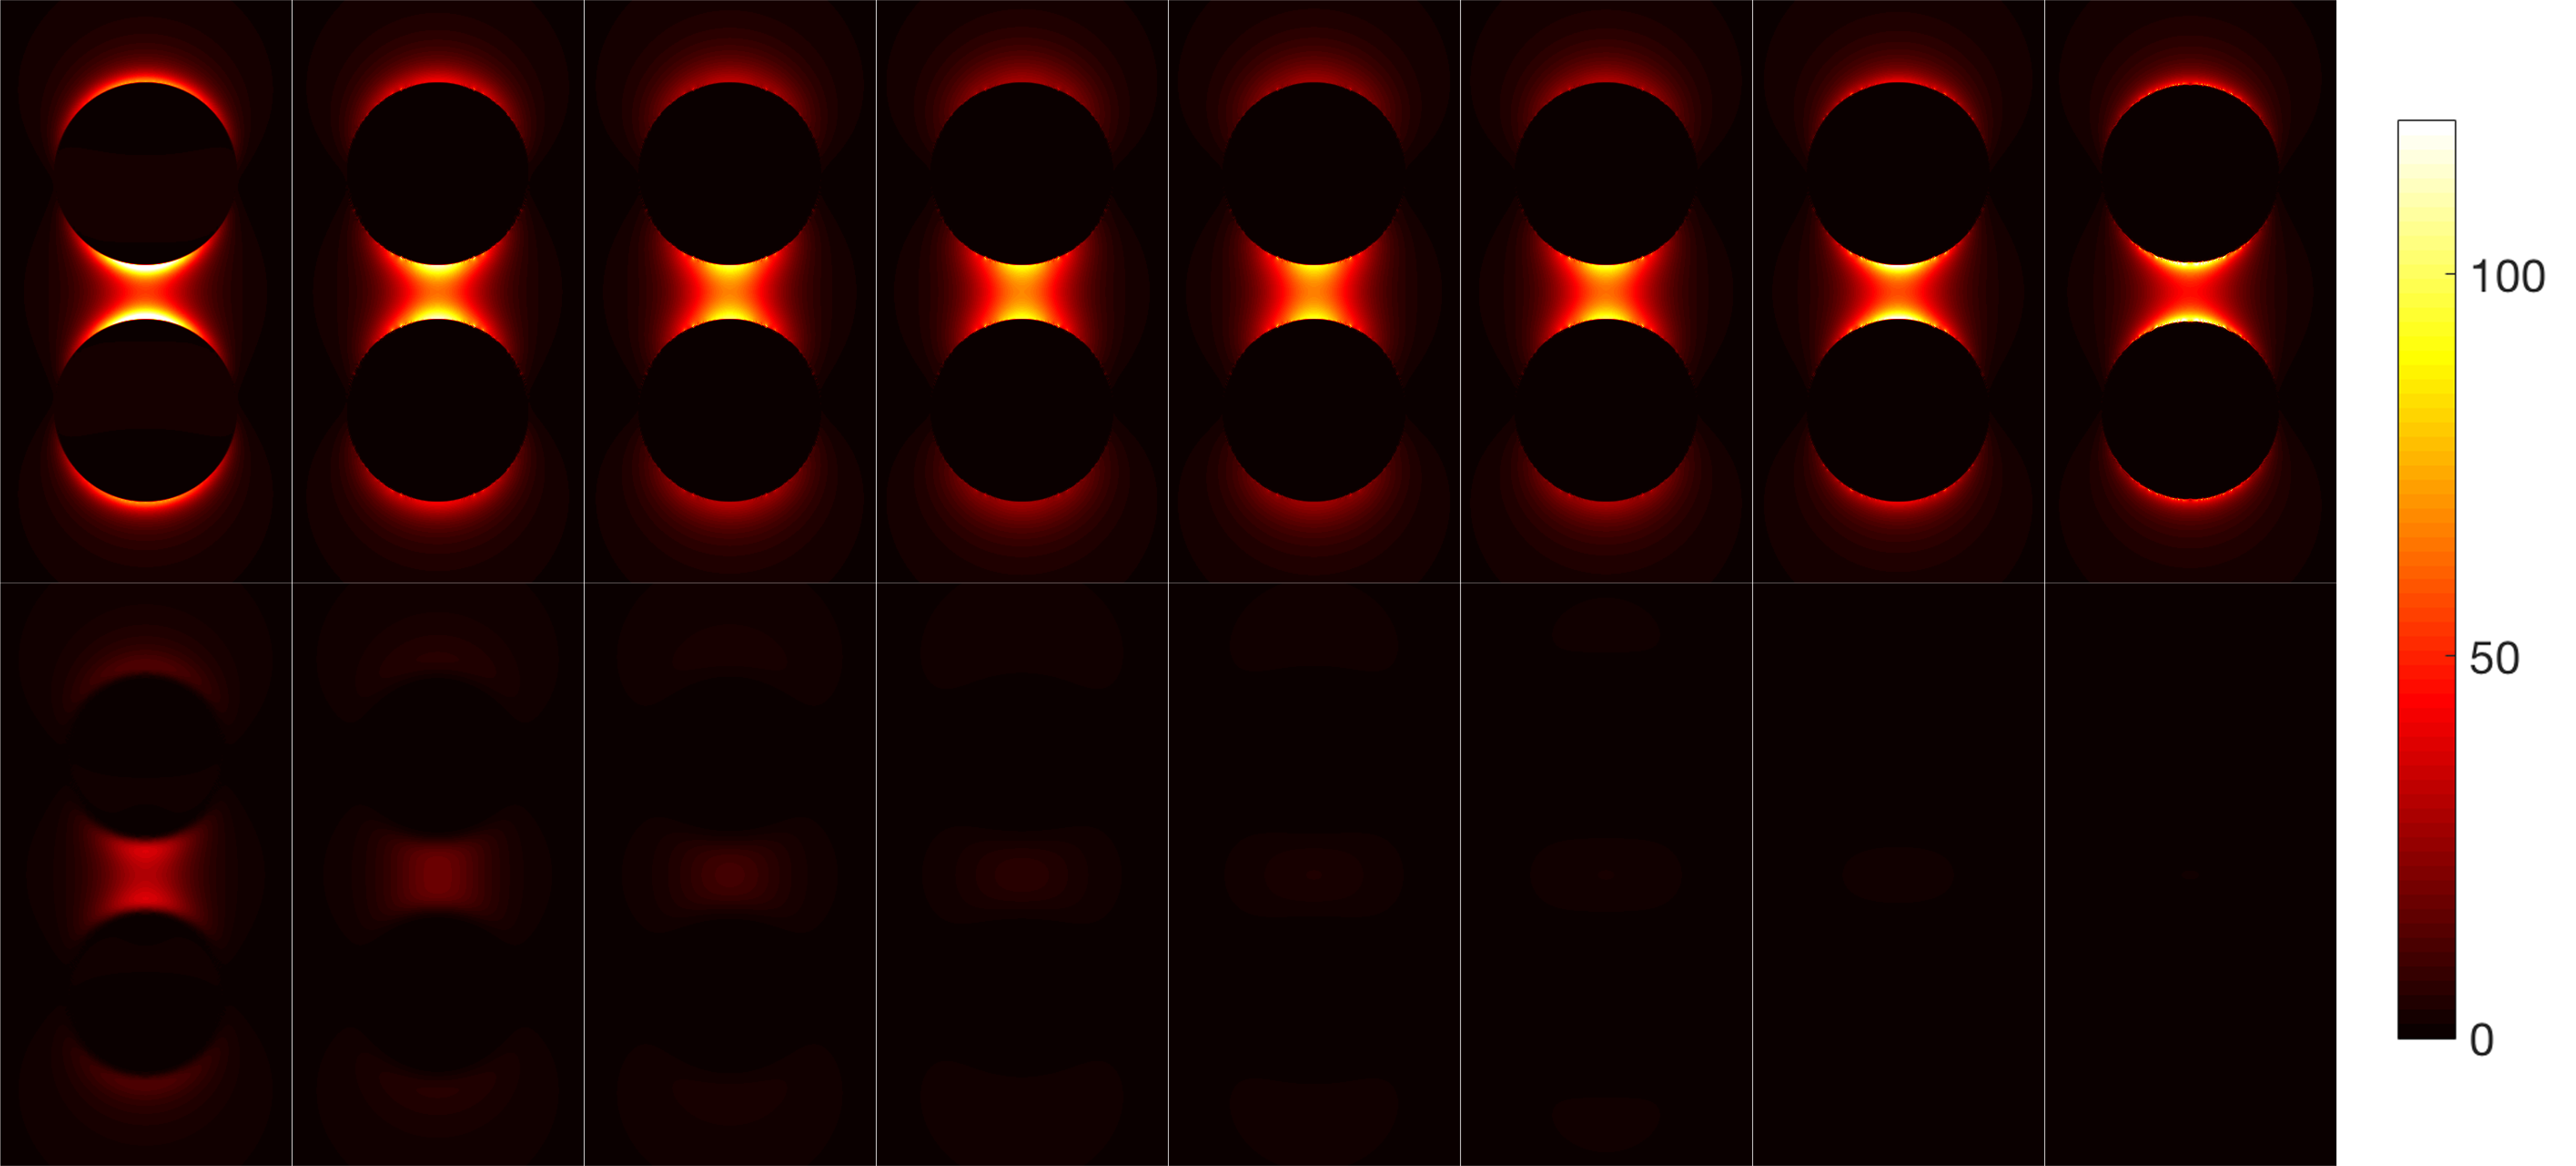
\includegraphics[width=\textwidth]{./images/simulation-slices.png}
  \caption{Slices of the simulation results in the $x y$-plane showing the near field enhancement $|E/E_0|^2$. Starting at the top left at $z=\SI{0}{nm}$ continuing in \SI{5}{nm} steps until $z=\SI{80}{nm}$.}
  \label{fig:slices}
\end{figure}
